
\documentclass[twocolumn]{article}

\newcommand{\Quip}{\texttt{Quip}}

\usepackage{dcj}
\usepackage{hyperref}
\usepackage{natbib}
\usepackage{graphicx}

\title{Compression of next-generation sequencing reads aided by highly efficient de novo assembly}
\author{Daniel C. Jones, Walter L. Ruzzo, Xinxia Peng, Michael G. Katze}

\begin{document}

\maketitle

\section{Abstract}

We present Quip, a compression algorithm for next-generation sequencing data
in the FASTQ and SAM/BAM formats. Reference-based compression is used to store
aligned reads compactly, as positions within an external sequence database.
Unaligned reads are further compressed by performing de novo assembly, and
storing sequences as positions within assembled contigs. To do so, we
developed a novel assembly algorithm which uses a probabilistic data structure
to greatly reduce the memory required by traditional De Bruijn graph
assemblers. This is combined with efficient statistical compression of read
identifiers, quality scores, alignment information, and sequences, effectively
collapsing very large datasets to less that 15\% of their original size.

Availability: Quip is freely available under an open-source license from
\url{http://cs.washington.edu/homes/dcjones/quip}.

\section{Introduction}

Next-generation sequencing (NGS) blah blah blah...

Disk storage costs have decreased dramatically over the past several decades
but have not kept track of 

A transformative breakthrough in storage technology may occur in the coming
years, but the age of the \$1000 genome is certain to arrive before that of
the \$100 petabyte hard disk. Futhermore, as cloud computing and software as a
service becomes increasingly relevant to molecular biology research, hours
spend transferring NGS datasets to and from off-site servers for analysis will
delay meaningful results. In some cases, researchers are forced to maximize
bandwidth by physically transporting storage media (colloquially, via the
``sneakernet''); an expensive and logistically complicated option. Even
moderate gains in domain-specific compression methods will translate into a
significant reduction in the cost of storage and management over time.

Storage and analysis of NGS data centers primarily around two formats that
have arisen as de facto standards: FASTQ and SAM/BAM. For its simplicity,
FASTQ is a surprisingly ill-defined format. The closest thing to an accepted
specification is the description by \citet{Cock2010}. The format arose ad hoc
from multiple sources (primarily Sanger and Solexa/Illumina), so this
specification in descriptive rather than prescriptive. The SAM format is far
more complex but also more tightly defined, and comes with a reference
implementation in the form of SAMtools \citep{Li2009b}. It is able to store
alignment information in addition to read identifiers, sequences, and quality
scores. Plain text, tab-delimited SAM files can also be converted to the BAM
format, a compressed binary version of SAM, which is far more compact and
allows for relatively efficient random access.

% DNA Compression

% NGS Compression

% Referenced-based compression

The fundamental characteristic of NGS data is that it consists of millions of
fragments of greater whole, whether it be a genome sequence or spliced mRNA
transcripts. This realization led \citet{Kozanitis2011} and \citet{Hsi-
YangFritz2011} to propose reference-based compression methods, in which reads
are aligned to a reference genome sequence, and the position with the genome
of each read is stored, rather than the read sequence itself. Decompression is
performed by copying the read sequences from the genome. Though any
differences from the reference sequence must also be stored, referenced-based
approaches can achieve much higher compression and they grow increasing
efficient with longer read lengths, since storing a genomic position requires
the same amount of space, regardless of the length of the read.

This idea is explored also in the Goby format \citep{Goby2012}, which has been
proposed an an alternative to SAM/BAM, the primary functional difference being
that sequences of aligned reads are not stored but looked up in a reference
genome when needed (frequently they are not). For some applications, reference-
based compression can be taken much further by storing only SNP information,
summarizing a sequencing experiment in mere kilobytes \citep{Christley2009}.
However, even when SNP calls are all that is needed, discarding the raw reads
would prevent any reanalysis of the data.


% Lossy compression of quality scores

A reoccurring theme in the  the growing literature on on short read
compression is lossy encoding of sequence quality scores. This follows
naturally from the realization that quality scores are particularly difficult
to compress. Unlike read identifiers, which are highly redundant, or
nucleotide sequences which XXX, quality scores are inconsistently encoded
between protocols and computational pipelines and are often simply high-
entropy. It is dissatisfying that metadata (quality scores) should consume
more space than primary data (nucleotide sequences). Yet, also dissatisfying
to many researchers is the thought of discarding information without a very
good understanding of its affect on downstream analysis.

A number of lossy compression algorithms for quality scores have been
proposed, including various binning schemes to reduce the alphabet size
\citep{Wan2011}, scaling to a reduced alphabet with randomized rounding
\citep{Kozanitis2011}, and discarding quality scores for bases which match a
reference sequence \citep{Hsi-YangFritz2011}. Only \citet{Kozanitis2011} go to
the effort of evaluating the effects of their algorithm on downstream
analysis. Their results suggest that while some SNP calls are affected, they
are primarily marginal, low-confidence calls between hetero- and homozygosity.

Decreasing the entropy of quality scores while retaining accuracy is an
important goal, but successful lossy compression demands an understanding of
what is lost. For example, lossy audio compression (e.g. MP3) is grounded in
psychoacoustic principles, preferentially discarding the least perceptible
sound. Conjuring a similarly principled method for NGS quality scores is
difficult given that both the algorithms that generate them and the algorithms
that are informed by them are moving targets. In the analysis by
\citet{Kozanitis2011}, the authors are appropriately cautious in interpreting
their results, pointing our that ``there are dozens of downstream applications
and much work needs to be done to ensure that coarsely quantized quality
values will be acceptable for users.''


% Quip to the rescue!

Though the method we propose here is entirely lossless, it is suitably general
(as is any method based on entropy encoding) so that any lossy transformation
applied upstream of compression can be automatically exploited.


\section{Methods}

\subsection{Statistical Compression with Arithmetic Coding}

Entropy encoding is a particularly elegant means of compression in that it
allows a distinct separation between modeling and encoding. In Quip, the same
arithmetic coder is used to encode quality scores, read identifiers,
nucleotide sequences, and alignment information, but with very different
statistical models for each.


\subsubsection{Read Identifiers}

The only requirement of read identifiers is that they uniquely identify the
read. A single integer would do, but typically each read comes with complex
string containing the instrument name, run identifier, flow cell identifier,
and tile coordinates. Much of this information is the same for every read and
is simply repeated, inflating the file size.

To compress out this redundancy, we use a form of delta encoding. A simple
parser tokenizes the ID into separate fields which are then compared to the
previous ID. Tokens that remain the same from read to read (e.g. instrument
name) and can be compressed to a negligible amount of space (arithmetic coding
produces codes of less than 1 bit for such tokens). Numerical token are
recognized and stored efficiently, either directly or as an offset from the
same token in the previous read. Otherwise the prefixes of non-identical
strings are matched before encoding the non-matching suffix.

The end result is that read IDs, which are often 50 bytes or longer, are
typically stored in 2-3 bytes.


\subsubsection{Nucleotide Sequences}

A large literature exists on compression DNA sequences. Genomes 
often contain regions of extreme redundancy and low complexity, but
with a structure that is complex and difficult to exploit.
%% TODO: a few comments on methods used throughout the ages

We however adopt a very simple model based on high-order Markov chains. The
nucleotide at a given position in a read is predicted using the preceding
twelve nucleotides. This model uses more memory than traditional general-
purpose compression algorithms ($4^{13} = 67,108,864$ parameters are needed,
each represented in 16 bits)  but it is simple and extremely efficient. An
order-12 Markov chain requires a very large amount of data to train , but
there is no shortage with sequencing data we wish to compress. After
compressing several million reads the parameters are tightly fit to the
nucleotide composition of the dataset so that the remaining reads will be
highly compressed. Compressing larger files only results in a tighter fit and
higher compression.


\subsubsection{Quality Scores}

It has been previously noted that the quality score at a given position is
highly correlated with the score at the preceding position
\citep{Kozanitis2011}. This makes a Markov chain a natural model, but unlike
nucleotides, quality scores are over a much larger alphabet (usually 41--46
distinct quality scores are used). This limits the order of the Markov chain:
long chains will require a great deal of space and take a unrealistic amount
of data to train.

To limit the number of parameters, we use an order-3 Markov chain, but
coarsely bin the distal two positions. In addition to the preceding three
positions, we condition on the position within the read and running count of
the number large jumps in quality scores between subsequent positions (defined
as $|q_{i} - q_{i-1}| > 1$), which allows reads with highly variable quality
scores to be encoded using a separate model. Both of these numbers are binned
to control the number of parameters.


\subsection{Reference-Based Compression}

We have also implemented lossless reference-based compression. Given aligned
reads in the SAM or BAM formats, and the sequence to which they are aligned
(in the FASTA format), the reads are compressed preserving all information in
the SAM/BAM file, including the header, read IDs, alignment information, and
all optional fields allowed by the SAM format.


\subsection{Assembly-Based Compression}

While a reference-based approach typically results in superior compression it
has a number of disadvantages. Most evidently, an appropriate reference
sequence database is not always available, particularly in the case of metagenomic
sequencing. One could beccontrived by compiling a set of genomes from species
expected to be represented in the sample. However, a high degree of expertise
is required to curate and manage such project-dependent a database. Secondly,
there is the practical concern that files compressed with a reference-based
approach are not self-contained. Decompression requires precisely the same
reference database used for compression, and if it is lost or forgotten the
compressed data becomes inaccessible.

To complement the reference-based approach, we developed an assembly-based
approach which offers some of the advantages of reference-based compression,
but requires no external sequence database and produces files which are
entirely self-contained. We use the first (by default) 2.5 million reads to
assemble contigs which are then used in place of a reference sequence
database to encode aligned reads compactly as positions.

Once contigs are assembled, read sequences are aligned using a simple ``seed
and extend'' method: 12-mer seeds are matched using a hash table, and
candidate alignments are evaluated using the Hamming distance. The best
(lowest Hamming distance) alignment is chosen, assuming it falls below a given
cutoff, and the read is encoded as a position within the contig set. Roughly,
this can be thought of as a derivation of the Lempel-Ziv algorithm: as
sequences are read, they are matched to previously observed data, or in this
case, contigs assembled from previously observed data. These contigs are
not explicitly stored, but rather reassembled during decompression.


% Probabalistic de bruijn graphs, etc

De novo assembly is traditionally extremely computationally intensive. The
most commonly used technique involves constructing a De Bruijn graph, a
directed graph in which each vertex represents a nucleotide $k$-mer present in
the data for some fixed $k$ (e.g., $k = 25$ is a common choice). An edge
between two $k$-mers $u$ and $v$ occurs if and only if the $(k-1)$-mer suffix
of $u$ is also the prefix of $v$. In principle, given such a graph, an
assembly can be produced by finding a path through this graph which follows
each edge exactly once, called an Eulerian path \citep{Pevzner2001}. In
practice, since NGS data has a non-negligible error rate, assemblers augment
each vertex with the number of observed occurrences of the $k$-mer and
leverage these counts using a variety of heuristics to filter out spurious
paths.

A significant bottleneck of the De Bruijn graph approach is building an
implicit representation of the graph by counting and storing $k$-mer
occurrences in a hash table. The assembler implemented in Quip overcomes this
bottleneck to a large extent by using a data structure based on the Bloom
filter to count $k$-mers. The Bloom filter \citep{Bloom1970} is a
probabilistic data structure that represents a set of elements extremely
compactly, at the cost of introducing a non-zero false positive rate. This
idea is generalized in the counting Bloom filter, in which an arbitrary count
can be associated with each element \citep{Fan2000}, and further refined in
the d-left counting Bloom filter (dlCBF) \citep{Bonomi2006}, which requires
significantly less space than the already quite space efficient counting Bloom
filter. We base our assembler on a realization of the dlCBF.

Counting $k$-mers efficiently with the help of Bloom filters was previously
explored by \citet{Melsted2011}, however it is used in addition, rather than
in place, of a hash table. The Bloom filter is used as a ``staging area'' to
store $k$-mers occurring only once, reducing the memory required by the hash
table. 

Concurrently with our work, \citet{Pell2011} have also developed a
probabilistic De Bruijn graph assembler but using a non-counting Bloom
filter. While they demonstrate a significant reduction in memory use, unlike
other De Bruijn graph assemblers, only the presence or absence of a k-mer is
stored, not its abundance, which is essential information when the goal is
producing accurate contigs. Nevertheless, their analysis suggests errors
introduced by false-positives in the Bloom filter are low when compared to
sequencing errors. This does not directly apply to the data structure used
here, but in Section \ref{section:dlcbf_results} we demonstrate that the
false-positive rate the dlCBF can be kept exceedingly low, while using a
little as an 20\% of the memory of a particularly space-efficient hash table.


\section{Results}
\label{section:results}

\subsection{Compression of Sequencing Data}

% Experiment setup

We compared Quip to three commonplace general-purpose compression algorithms:
gzip, bzip2, and xz, as well as more recently developed domain-specific
compression algorithms: DSRC \citep{Deorowicz2011} and Cramtools \citep{Hsi-
YangFritz2011}. Other methods have been proposed \citep{Tembe2010,
Kozanitis2011, Bhola2011, Sakib2011}, but without publicly available software
we were unable independently evaluate them. We have also restricted our focus
to lossless compression, and have not evaluated a number of promising lossy
methods \citep{Hsi-YangFritz2011,Wan2011,Hach2012}. We acquired six datasets
(Table \ref{tab:datasets}) from the Sequence Read Archive
\citep{Leinonen2011}, representing a broad sampling of recent applications of
next-generation sequencing.

The Sequence Read Archive provides data in its own SRA compression format
which we also evaluate here. Programs for working with SRA files are provided
in the SRA Toolkit, but a convenient means of converting from FASTQ to SRA is
not provided, so we have not measured compression time and memory in this
case.

% Evaluating reference based compression

In the case of reference based alignment implemented in Cramtools and Quip, we
aligned reads from all but the metagenomic data to the GRCh37/hg19 assembly of
the human genome using Gsnap generating a BAM file. Splice-junction prediction
was enabled for the two RNA-Seq datasets. In the case of multiple alignments,
we removed all but the the primary (i.e., highest scoring). Quip is able to
store secondary alignments, but the version of Cramtools we evaluated was not.
When the purpose of alignment in simply compactly archiving the the reads,
secondary alignments have no purpose and merely inflate the file size, but in
downstream analysis they are often extremely informative and retaining them
may be desirable in some cases.

% Cramtools is not lossless! It has a big advantage and is still losing.

It is important to note that lossless compression is not the intended goal of
Cramtools. Though we invoked Cramtools with options to include all quality
scores (\texttt{--capture-all-quality-scores}), optional tags (\texttt
{--capture-all- tags}), and retain unaligned reads (\texttt{--include-
unmapped-reads}), it is unable to store the original read IDs. This puts it at
advantage when comparing compressed file size, as all other programs compared
were completely lossless, but as the only other available reference-based
compression, it is a useful comparison.


% Reference-based compression of metagenomic data is not a very good idea.

We do not attempt reference-based compression of the metagenomic data; it is
more diffilult and less practical than doing so for single-genome data. In
nonspecific metagenomic sequencing, there is typically no obvious reference
sequence database. One could be contrived by compiling a set of genomes of
species expected to be represented in the sample. However, with no consistent,
accepted standard reference, the compressed data could easily become
inaccessible if the reference used for compression is lost. Furthermore a high
degree of expertise is needed to curate such a project-dependent reference.

% Measurements

With each method we compressed then decompressed each dataset on a server with
a 2.8Ghz Intel Xeon processor and 64 GB of memory. In addition to recording
the compressed file size (Figure \ref{fig:sizes}), we measured absolute run-
time (Figure \ref{fig:comp_decomp_time}) and maximum memory usage (Table
\ref{tab:mem_usage}) using the Unix \texttt{time} command.

In the single-genome samples, we find that reference-based compression using
Quip consistently results in the smallest file size (i.e., highest
compression). Indeed, in three datasets, we achieve higher compression without
the use of a reference sequence. Despite using a similar reference-based
scheme and discarding read identifiers, compression with Cramtools results in
significantly larger file size. This is due in part to different encoding
algorithms: Quip uses arithmetic coding while Cramtools uses Huffman and
Golomb coding. But the models used in both are, as a whole, complex and very
different, so accounting for this difference in file size is non-trivial.

Assembly-based compression provides almost no advantage in the single-genome
ChIP-Seq, Whole Genome, and Exome datasets. Because we assembly only several
million reads (2.5 million, by default), coverage is only enough to assembly
representatives of certain families of repeats in these datasets.

In the RNA-Seq datasets, more is assembled (approximately XXX\% and 70\% of
the reads are aligned to assembled contigs in the total RNA-Seq and mRNA-Seq
datasets, respectively), but this only provides a small increase in the
compression. When a read is not aligned, it is compressed with a high-order
Markov chain model. The Markov chain and assembly-based compression methods
both benefit from low-entropy data. Thus, reads that are aligned to contigs
are disproportionately low-complexity, explaining why the compression gains
are small despite so much being assembled: though many reads deriving from
repeats are stored as alignments, these reads are low-complexity and would
have been stored only slightly less compactly with a high-order Markov chain.

Nevertheless, assembly-based compression does provide a significant advantage
in the metagenomic dataset. Nearly 95\% of reads align to assembled contigs,
resulting in a large reduction in compressed file size. Though this may be the
result of low species diversity and may not extend to all metagenomic
datasets, it shows that assembly-based compression is beneficial in certain
cases. Though it comes at some cost, we are able to perform assembly with
exceedingly  high efficiently: compression time is faster than all but DSRC
and assembly-free Quip even while assembling 2.5 million reads and aligning
millions more reads to the assembled contigs, and memory usage is increased by
only 400 MB.


\begin{table}
%% TODO: list versions as well
\begin{tabular}{lp{0.3\textwidth}}
\textit{Method} & \textit{Description} \\ \hline
gzip (1.4)      & General-puprose Lempel-Ziv \\
bzip2 (1.0.6)   &
General-purpose Burrows-Wheeler transformation and Huffman coding \\
xz  (5.0.3)     &
General-purpose Lempel-Ziv and arithmetic coding \\
sra (2.1.10)           & No published description \\
dsrc (0.3) & Markov chains,  with Huffman coding \\
cramtools (0.85-b51)  & Referenced-based, \\
quip            & Arithmetic coding \\
quip -a         & Quip with assembly-based compression \\
quip -r         &
Quip with reference-reference based compression \\
\end{tabular}
\caption{Methods evaluated in Section \ref{section:results}.
All methods compared are lossless, with the exception of cramtools which
does not preserve the original read identifiers.}
\label{tab:methods}
\end{table}


\begin{table}
\begin{tabular}{rllr}
  & \textit{Accession Number} & \textit{Description} & \textit{Size (GB)} \\ \hline
1 & SRR400039                 & Whole Genome         & 67.6 \\
2 & SRR125858                 & Exome                & 55.2 \\
3 & ERR030867                 & Total RNA            & 19.5 \\
4 & SRR372816                 & Runx2 ChIP-Seq       & 14.6 \\
5 & ERR030894                 & mRNA                 & 16.4 \\
6 & SRR359032                 & Metagenomic DNA      &  8.9 \\
\end{tabular}
\caption{
We evaluated compression on a single lane of sequencing data taken from a
broad collection of seven studies. Except for the metagenomic data, each was
generated from human samples. File size is shown in gigabytes.
}
\label{tab:datasets}
\end{table}


\begin{figure*}
\centerline{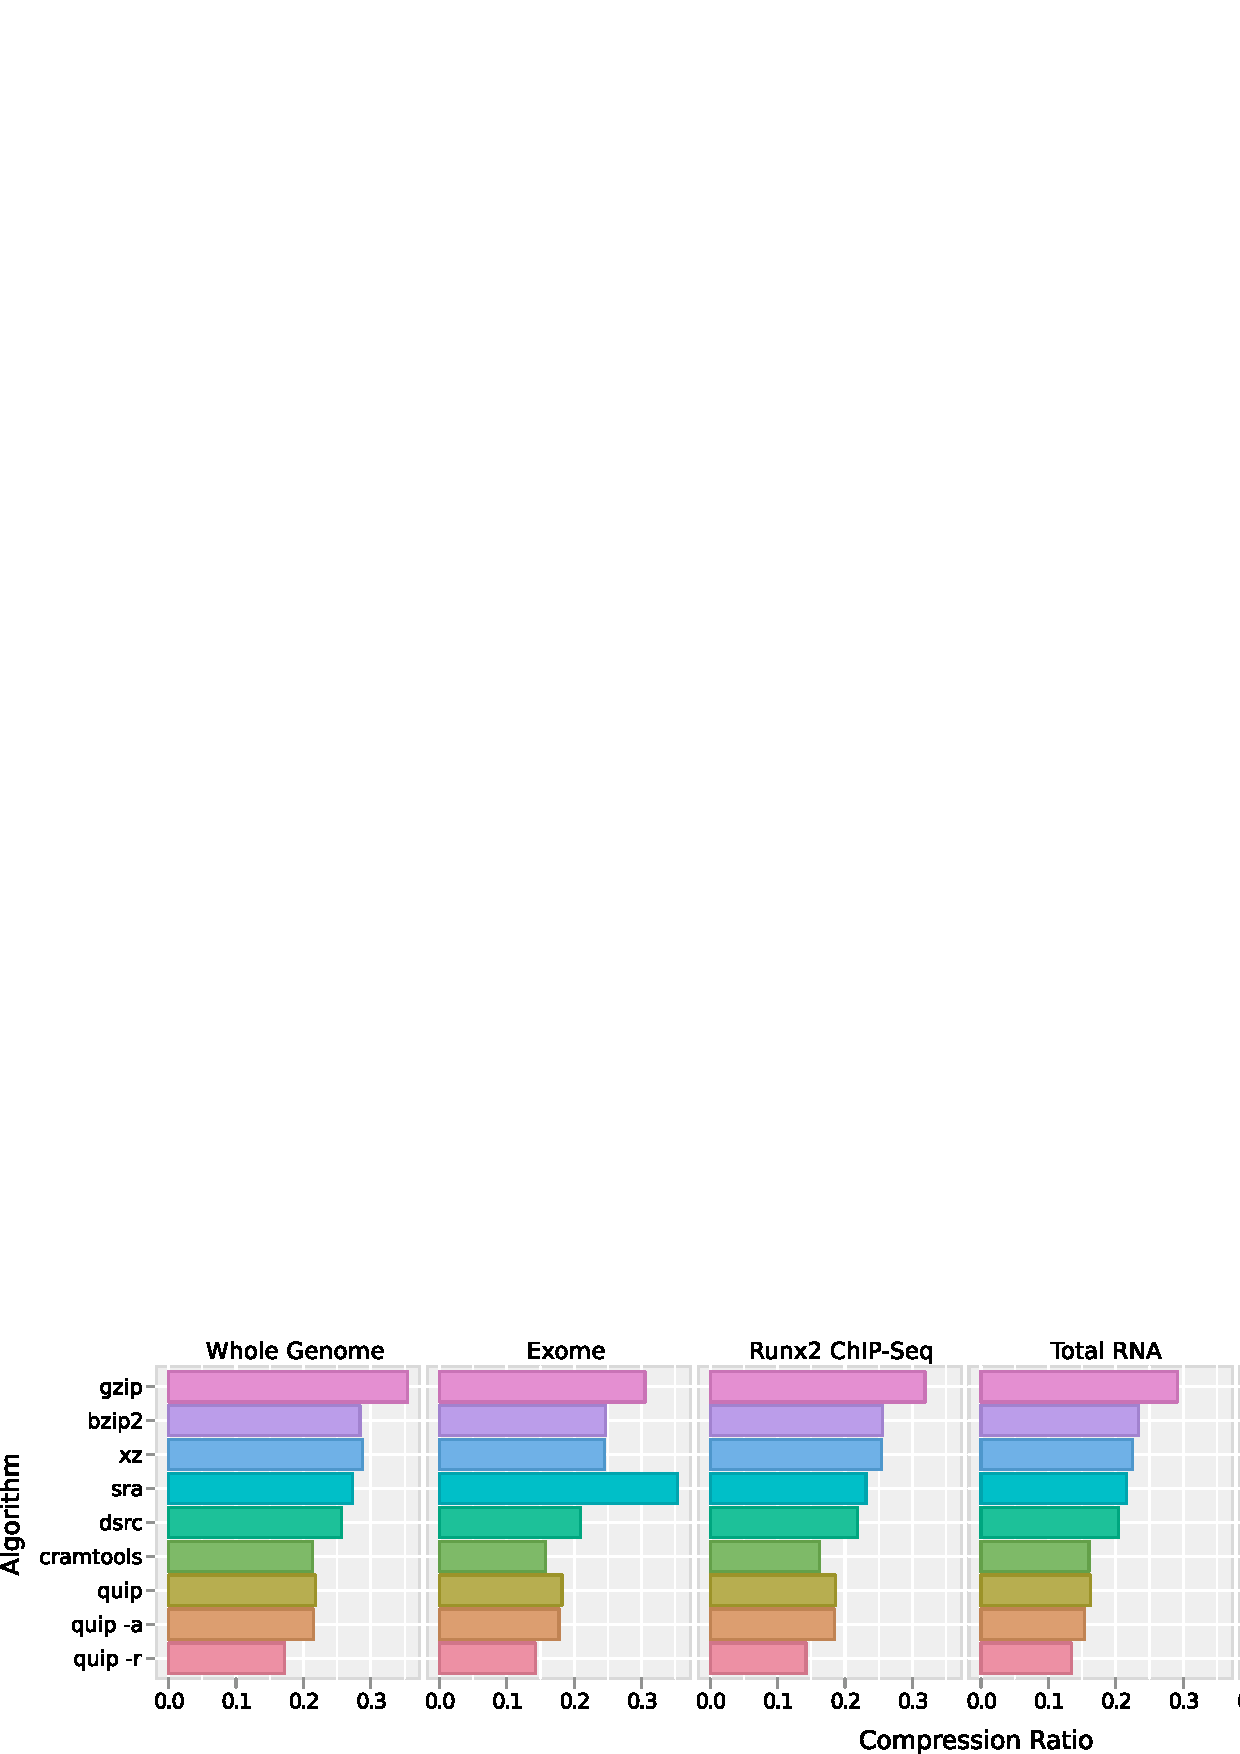
\includegraphics[width=\textwidth]{analysis/sizes.pdf}}
\caption{
A single lane from six sequencing experiments was compressed using each
method. The size of each compressed file is plotted in proportion to the
uncompressed file size. Reference-based compression methods were not applied to
to the metagenomic dataset. These plots are marked ``NA''.
}
\label{fig:sizes}
\end{figure*}

\begin{figure*}
\centerline{\includegraphics[width=\textwidth]{analysis/comp_time.pdf}}
\centerline{\includegraphics[width=\textwidth]{analysis/decomp_time.pdf}}
\caption{
The absolute run time of each evaluation was recorded using the Unix time
command. Compression speed in measured in megabytes of input per second, while
the decompression speed is in megabytes of output per second. In the case of
the reference-based compressors, cramtools and quip -r, output is in the BAM
format and so these measurements include time spend re-compressing the data
with zlib.
}
\label{fig:comp_decomp_time}
\end{figure*}

\begin{table}
\centerline{
\begin{tabular}{lrr}
                & \multicolumn{2}{c}{\textit{Average Memory Usage (MB)}} \\ \cline{2-3}
\textit{Method} & \textit{Compression} & \textit{Decompression} \\ \hline
gzip            &     0.8              &    0.7 \\
bzip2           &     7.0              &    4.0 \\
xz              &    96.2              &    9.0 \\
sra             &      NA              &        \\
dsrc            &    28.3              &   15.1 \\
cramtools       &  6803.8              & 6749.3 \\
quip            &   412.1              &  412.9 \\
quip -a         &   823.0              &  794.1 \\
quip -r         &  1717.0              &
\end{tabular}
}
\caption{
Maximum memory usage was recorded for each program and dataset. We list
the average across datasets of these measurements. For most of the programs,
memory usage was near constant across datasets. The largest variance was seen
with Cramtools and Quip with de novo assembly (``quip -a''). Cramtools varied
between 9.2 GB and 11.5 GB during compression, and from 8.8 to 10.8 GB during
decompression. Quip varied from 808 to 931 MB in compression and
decompression when run with de novo assembly.
}
\label{tab:mem_usage}
\end{table}


\subsection{Characteristics of the d-left Counting Bloom Filter}

\label{section:dlcbf_results}

Though our primary goal is efficient compression of sequencing data, the
assembly algorithm we developed to achieve this is of independent interest.
Only very recently has the idea of using probabilistic data structures in
assembly been breached, and to our knowledge, we are the first to build
a functioning assembler using any version of the counting Bloom filter.

The precise false positive rate of the dlCBF data structure is unimportant
when the goal is compression, but if the method is to be extended to perform
actual analysis, it becomes a serious concern. The false positive rate of a
Bloom filter can be obtained analytically, though doing so is not entirely
trivial.
%% TODO: can the dlCBF false-positive rate be obtained analystically?

Comparisons of data structure performance are notoriously sensitive to the
particulars of the implementation. To perform a meaningful benchmark, we
compared our dlCBF implementation to the sparsehash library, an open source
hash table implementation with the expressed goal of maximizing space
efficiency. Among many other uses, it is the core data structure in the ABySS
\citep{Simpson2011} and PASHA \citep{Liu2011} assemblers.

We randomly generated 10 million unique 25-mers and inserted them into a hash
table sized appropriately as to avoid expansion and rehashing. We repeated
this with dlCBF tables of increasing sizes. Upon insertion, a false positive
occurs when the hash functions computed on the inserted $k$-mer collide with a
previously inserted $k$-mer. An insertion may also fail when a fixed size
table is filled to capacity and no empty cells are available. For simplicity,
we count these occurrences also as ``false positives''. Run time and maximum memory
usage were both recorded using the Unix time command.

\begin{figure}[h]
\centerline{\includegraphics[width=0.5\textwidth]{analysis/dlcbf/benchmark.pdf}}
\caption{
The trade-off between memory usage and false positive rate in the dlCBF is
evaluated by inserting 10 million unique 25-mers into tables of increasing
size. Memory usage in reported as the proportion of the memory used by a
memory efficient hash table to do the same.
}
\label{fig:dlcbf_bench}
\end{figure}

We find that with only 20\% of the space of the hash table the dlCBF accrues a
false positive rate of less than 0.001 (Figure \ref{fig:dlcbf_bench}). While
the hash table performed the 10 million insertions in 7.34 seconds, it
required only 0.61 seconds on average for the dlCBF to do the same on a 2.8Ghz
Intel Xeon processor. Table size did not greatly affect the runtime of the
dlCBF.

Though the authors of sparsehash claim only a 4 bit overhead for each entry,
and have gone to considerably effort to achieve such efficiency, it still must
store the $k$-mer itself, encoded in 64 bits. The dlCBF avoids this, storing
instead a 14-bit ``fingerprint'', or hash of a $k$-mer, resulting in the large
savings we observe. Of course, a 25-mer cannot be uniquely identified with 14
bits. False positives are thus introduced, yet they are kept at a very low
rate by the d-left hashing scheme. Since multiple hash functions are used
under this scheme, multiple collisions must occur to result in a false
positive; an infrequent event if reasonably high-quality hash functions are
chosen.

A previous analysis of the dlCBF by \citet{Zhang2009} compared it to two other
variations of the counting Bloom filter and concluded that ``the dlCBF
outperforms the others remarkably, in terms of both space efficiency and
accuracy.'' Overall, this data structure appears particularly adept for high
efficiency de novo assembly.

\section{Discussion}

Compared to the only other published and freely-available reference-based
compressor, Cramtools, we see a significant reduction in compressed file size,
despite read identifiers being discarded by Cramtools and retained by Quip.
This is combined with dramatically reduced memory usage, faster compression
and decompression, and increased flexibility (e.g. Quip is able to store
multiple alignments of the same read and does not require that the BAM file be
sorted or indexed). Conversely, Cramtools implements some potentially very
useful lossy methods not provided by Quip. For example, a number of options
are available for selectively discarding quality scores that are deemed
unnecessary.

%% Points to make
% We are doing de novo assembly faster than gzip can compress!!
% DSRC support random access, but there is never a need for this with FASTQ.

% Lempel-Ziv is ill-suited to NGS data

The Lempel-Ziv algorithm, particularly as implemented in gzip/libz has become
a reasonable default choice for compression. The zlib library has matured and stabilized
over the course of two decades and is widely available. The BAM and Goby
formats both use zlib for compression, and compressing FASTQ files with gzip
is still common practice. Despite its ubiquity, our benchmarks show that it is
remarkably poorly suited to NGS data. Both compression ratio and compression
time were inferior to the other programs evaluated. For most purposes, the
gains in decompression time do not make up for its shortcomings.

Using a more sophisticated variation, the Lempel-Ziv-Markov algorithm
implemented in xz results in a significant increase in compression, but at the
cost of tremendously slow compression (often an entire day is required to
compress a single lane from a HiSeq 2000). This is not a great surprise: the
Lempel-Ziv algorithm works by matching repeated substrings in the input
stream; This is an extremely effective technique for compressing text, but
when the data is not so highly structured, as is the case with quality scores,
it breaks down.

%% Something else here?


% Memory/Time Usage

Our use of high-order Markov chain models and de novo assembly results in a
program that uses significantly more memory than the others tested, with the
exception of cramtools. Though limiting the memory used by a general purpose
compression program enables it to be used on a wider variety of systems, this
is less important in this domain-specific application. Common analysis of
next-generation sequencing data, whether it be alignment, assembly, isoform
quantification, peak calling, or SNP calling all require significant
computational resources. Targeting low-memory systems would not be of
particular benefit: next-generation sequencing precludes previous-generation
hardware.

Though memory consumption is not a top priority, runtime is important. Newer
instruments like the HiSeq 2000 produce far more data per lane than previously
possible. And, as the cost of sequencing continues to decrease, experiments
will involve more conditions, replicates, and timepoints.  Quip is able to
compress NGS data at three times the speed of gzip, while performing de novo
assembly of millions of reads, and up to five times as fast without the
assembly step. Only DSRC is faster, but with consistently lower compression.
In addition, our reference-based compression algorithm is nearly twice as fast
as cramtools, with substantially better lossless compression.

% Conclusion

The algorithm implemented in Quip combines an ensemble of powerful techniques
to probe the limit to which next-generation sequencing data can be compressed,
yet remains efficient enough to be practical.

\section*{Acknowledgments}

James Bonfield, Matt Mahoney, Seth Hillbrand

% TODO: Etc.

\bibliographystyle{plainnat}
\bibliography{quip}

\end{document}



